\documentclass{article}

\usepackage[compat=1.1.0]{tikz-feynman}

\begin{document}

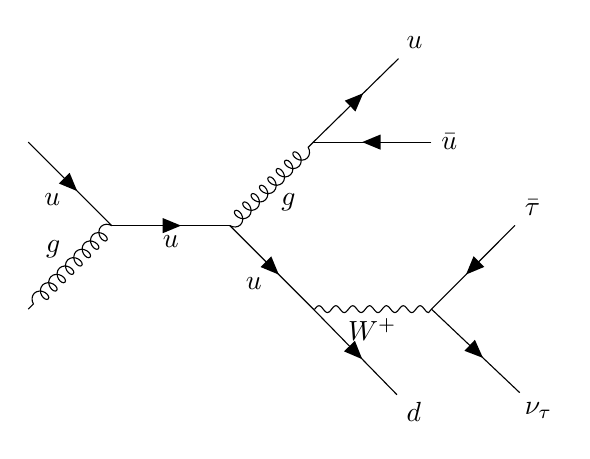
\begin{tikzpicture}
	\begin{feynman}
		\vertex (a);
		\vertex [below right=of a] (b);
		\vertex [below left=of b] (c);
		\vertex [right=of b] (d);
		\vertex [above right=of d] (e);
		\vertex [above right=of e]  (h) {\(u\)};
		\vertex [right=of e] (g) {\(\bar{u}\)};
		\vertex [below right=of d] (i);
		\vertex [below right=of i] (l) {\(d\)};
		\vertex [right=of i] (m);
		\vertex [above right=of m] (n) {\(\bar{\tau}\)};
		\vertex [below right=of m] (o) {\(\nu_{\tau}\)};
		

		\diagram* {
			(a) -- [fermion, edge label'=\(u\)] (b) -- [fermion, edge label'=\(u\)] (d);
			(b) -- [gluon, edge label'=\(g\)] (c);
			(d) -- [gluon, edge label'=\(g\)] (e);
			(g) -- [fermion] (e) -- [fermion] (h);
			(d) -- [fermion, edge label'=\(u\)]  (i) -- [fermion] (l);
			(i) -- [boson, edge label'=\(W^{+}\)] (m);
			(n) -- [fermion] (m) -- [fermion] (o);
			
		};
		
	\end{feynman}	
	
\end{tikzpicture}

\bigbreak
\bigbreak
\bigbreak

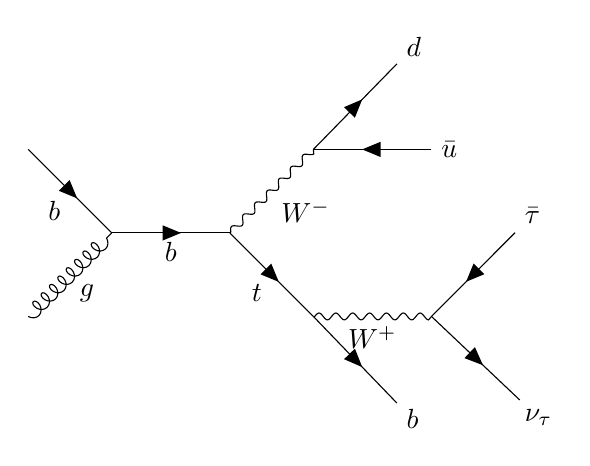
\begin{tikzpicture}
	\begin{feynman}
		\vertex (a);
		\vertex [below right=of a] (b);
		\vertex [below left=of b] (c);
		\vertex [right=of b] (d);
		\vertex [above right=of d] (e);
		\vertex [above right=of e] (f) {\(d\)} ;
		\vertex [right=of e] (g) {\(\bar{u}\)};
		\vertex [below right=of d] (h);
		\vertex [below right=of h] (i) {\(b\)};
		\vertex [right=of h] (l);
		\vertex [above right=of l] (m) {\(\bar{\tau}\)};
		\vertex [below right=of l] (n) {\(\nu_{\tau}\)};
	
		\diagram* {
			(a) -- [fermion, edge label'=\(b\)] (b) -- [fermion, edge label'=\(b\)] (d);
			(c) -- [gluon, edge label'=\(g\)] (b);
			(d) -- [boson, edge label'=\(W^{-}\)] (e);
			(g) -- [fermion] (e) -- [fermion] (f);
			(d) -- [fermion, edge label'=\(t\)] (h) -- [fermion] (i);
			(h) -- [boson, edge label'=\(W^{+}\)] (l);
			(m) -- [fermion] (l) -- [fermion] (n);
	}	;
	\end{feynman}
\end{tikzpicture}	

\bigbreak
\bigbreak
\bigbreak

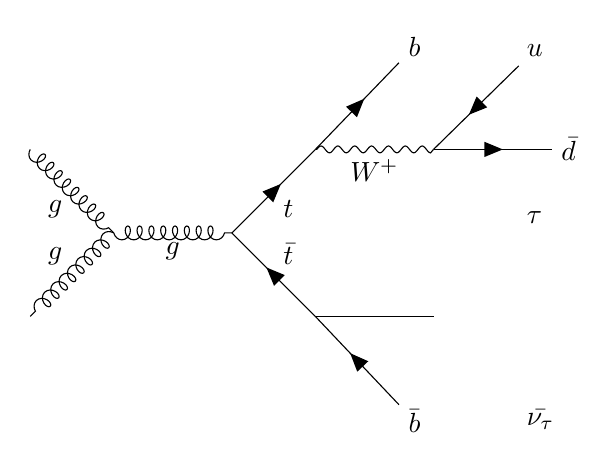
\begin{tikzpicture}
\begin{feynman}
\vertex (a);
\vertex [below right=of a] (b);
\vertex [below left=of b] (c);
\vertex [right=of b] (d);
\vertex [above right=of d] (e);
\vertex [above right=of e] (f){\(b\)};
\vertex [right=of e] (g);
\vertex [above right=of g] (h) {\(u\)};
\vertex [right=of g] (i) {\(\bar{d}\)};
\vertex [below right=of d] (l);
\vertex [below right=of l] (m){\(\bar{b}\)};
\vertex [right=of l] (o);
\vertex [above right=of o] (p){\(\tau\)};
\vertex [below right=of o] (q){\(\bar{\nu_{\tau}}\)};

\diagram* {
(a) -- [gluon, edge label'=\(g\)] (b) -- [gluon, edge label'=\(g\)] (c);
(b) -- [gluon, edge label'=\(g\)] (d);
(d) -- [fermion, edge label'=\(t\)] (e) -- [fermion] (f);
(h) -- [fermion] (g) -- [fermion] (i);
(e) -- [boson, edge label'=\(W^{+}\)] (g);
(m) -- [fermion] (l) -- [fermion, edge label'=\(\bar{t}\)] (d);
(l) -- (o)
}	;
\end{feynman}
\end{tikzpicture}	

\end{document}
